% Persuasiveness Scorer Section
\section{Prototype-then-Edit For Control}
\label{sec:neural_editor}

In this section, we detail our work extending the prototype-then-edit framework proposed by \citet{guu2018generating} to include a fine-grained control on speed. We provide some background context in~\Cref{subsec:ne_background} and then present the main prototype-then-edit model in~\Cref{subsec:ne_model}. We propose two novel modifications to the framework for controllable generation in~\Cref{subsec:ne_methodology}. Then in~\Cref{subsec:ne_exp_settings}, we describe the experimental settings, baselines, and metrics. Lastly, in~\Cref{subsec:ne_results}, we present the results of our modifications.

\subsection{Background}
\label{subsec:ne_background}

\citet{guu2018generating} introduce a novel unconditional generative model that samples a ``prototype'' sentence from the training corpus and edits it using a randomly sampled edit vector. The authors find that within the Yelp restaurant review corpus, 70\% of the test set is within a Jaccard distance of 0.5 of a training set sentence, implying that a neural editor with smooth and consistent edits should capture the test set. There are two significant constraints for the edit model:
\begin{itemize}
    \item \textbf{Semantic Smoothness}: Edits should change the semantics of a sentence by a small amount and, when stacked together, create a larger change.
    \item \textbf{Consistent Edit Behavior}: The edit vector, $z$, should control the change in a sentence such that when applied to different sentences, the edits are semantically analogous.
\end{itemize}

\subsection{Prototype-then-edit Model}
\label{subsec:ne_model}

We provide details into how \citet{guu2018generating} define their model. The likelihood of a sentence is formulated as:

\begin{equation}
p(x) = \sum_{x' \in \mathcal{X}} p(x | x') p(x')    
\end{equation}

where $x'$ is prototype sentence, $x$ is the generated sentence, and  $p(x | x') = \mathbb{E}_{z \sim p(z)} [p_{edit}(x | x', z)]$. However, since this requires a sum over all prototypes $x'$, the authors only sum over the $x'$ that are lexically similar to $x$. They create a lexical similarity neighborhood:

\begin{equation}
\mathcal{N}(x) = \{x' \in \mathcal{X} : d_J(x, x') < 0.5\}
\end{equation}

where $d_J$ is the Jaccard distance. The model is trained by maximizing the marginal likelihood, $p(x)$, with gradient ascent. However, $p(x|x')$ has no closed-form solution, which is solved by lower bounding the expectation with the evidence lower bound (ELBO) \citep{kingma2013auto}. 

Ultimately, the model features three main components: a neural editor $p_{edit}(x | x', z)$, an inverse neural editor $q(z | x', x)$, and an edit prior $p(z)$. The neural editor and inverse neural editor combine to form a VAE. The neural editor is a sequence-to-sequence model with attention, where given $x'$ as input and $z$, which is concatenated to the input of the decoder at each step, it generates $x$. The edit vector is $z = z_{norm} \cdot z_{dir}$ where $z_{norm}$, the strength of the edit, is drawn from $\mathcal{U}(0,10)$ and $z_{dir}$, the direction of the edit, is sampled from a uniform distribution on the unit sphere. The inverse neural editor is given the edit pair $(x, x')$ and must infer the edit vector $z$. The difference between $x$ and $x'$ is represented as

\begin{equation}
    f(x, x') = \sum_{w \in I} \Phi(w) \oplus \sum_{w \in D} \Phi(w)
\end{equation}

where $I = x \setminus x'$ (\ie the set of words added to $x'$), $D = x \setminus x'$ (\ie the set of words deleted from $x'$), and $\Phi(w)$ is the GloVe \citep{pennington2014glove} vector for $w$. The inverse neural editor outputs a perturbed version of $f(x, x')$ as the edit vector, as follows:

\begin{equation}
q(z_{dir} | x', x) = \text{vMF}(f_{dir}, \kappa)
\end{equation}
\begin{equation}
q(z_{norm} | x', x) = \mathcal{U}(f_{norm}, f_{norm} + \epsilon)
\end{equation}

where $f_{norm} = \min(\|f\|, 10 - \epsilon)$ and $f_{dir} = \frac{f}{f_{norm}}$. Let $\text{vMF}(\mu, \kappa)$ be a von-Mises Fisher distribution where $\mu$ is the mean vector, and $\kappa$ is the concentration parameter\footnote{$\kappa$ controls the rate of decay as the log-likelihood of a point decays linearly with the cosine similarity to $\mu$ in vMF distributions}.

\subsection{Controlling Edits}
\label{subsec:ne_methodology}

In order to introduce a control mechanism for speed, we target two aspects of the prototype-then-edit model: neighborhood creation and edit vector perturbation.

\textbf{Neighborhood Creation}: The model's behavior is heavily constrained by the lexical similarity condition in the creation of the neighborhood. By creating an additional constraint on speed, we can ensure that edit vectors drawn from $p(z)$ correspond to a specified change in speed. More formally, we define the neighborhood as

\begin{equation}
\mathcal{N}_{\Delta}(x) = \{x' \in \mathcal{X} : d_J(x, x') < 0.5, |(s(x) - s(x')) - \Delta| \leq \epsilon \}
\end{equation}

where $s(\cdot)$ is the speed of a text, $\delta$ is a desired change in speed, and $\epsilon$ is some tolerance. Note that the direction of speed is enforced with $(s(x) - s(x'))$.

\textbf{Edit Vector Peturbation}: We hypothesize that by altering the magnitude of $z_{norm}$ and the direction $z_{dir}$, we can control the strength and behavior of the edit vector. Expressly, we can condition the formulation of the inverse neural editor on speed by defining $q(z_{norm} | x', x) = \mathcal{N}(\Delta, 1) \cdot \mathcal{U}(f_{norm}, f_{norm} + \epsilon)$, where $\mathcal{N}$ is the normal distribution, $\mathcal{U}$ is the uniform distribution, and $\Delta$ is the desired change in speed.

\subsection{Experimental Settings}
\label{subsec:ne_exp_settings}

We train multiple variants of the edit-then-prototype model on the Yelp Restaurant Reviews Corpus\footnote{Formerly, \url{https://www.yelp.com/dataset/challenge}}:

\textit{\textbf{\textsc{NeuralEditor} Baseline}} We use the out-of-the-box model to provide a baseline on sequence-to-sequence evaluation metrics as well as a baseline $\Delta$.

\textit{\textbf{Neighborhood Creation}} We add the $\Delta$ constraint during neighborhood creation and train on the newly formed data. We try $\epsilon = \{0.05, 0.1, 0.2\}$ as tolerance values.

\textit{\textbf{Perturbation}} We add the $\Delta$-centered normal distribution to perturb the edit vector during training.

\textit{\textbf{Perturbation \& $\Delta$-Tolerance}} We combine the previous two approaches, again testing $\epsilon = \{0.05, 0.1, 0.2\}$.

All hyperparameters are left the same as in the original paper \citep{guu2018generating}. We record a few evaluation metrics to test the strength of the control as well as to ensure generations are not too different:

\textit{\textbf{Delta}} We record the learned change in speeds (\ie $\Delta$).

\textit{\textbf{BLEU}} We measure the n-gram overlap (lexical similarity) through BiLingual Evaluation Understudy (BLEU) scores \citep{Papineni2002bleu} for both the training and test sets. 

\textit{\textbf{BERTScore}} We measure the semantic similarity through the BERTScore \citep{zhang2019bertscore} to ensure that generations remain on topic.

\subsection{Results}
\label{subsec:ne_results}

We analyze the distribution of $\Delta$ (\ie change in speed) in $\mathcal{N}(x)$ in~\Cref{fig:ne_speed_distr}. The distribution is centered at 0 and denser at smaller magnitudes of $\Delta$, implying a lack of training data for larger shifts in speed. We will discuss this limitation later.

\begin{figure*}[t]
  \centering
  \caption{Histogram of delta values (\ie $s(x) - s(x')$) within the Yelp Restaurant Review Corpus. The x-axis represents the difference in speed within the pairs of our created neighborhood, $\mathcal{N}(x)$, without any constraint on speed. The y-axis counts the number of pairs exhibiting the given delta in log-scale.}
  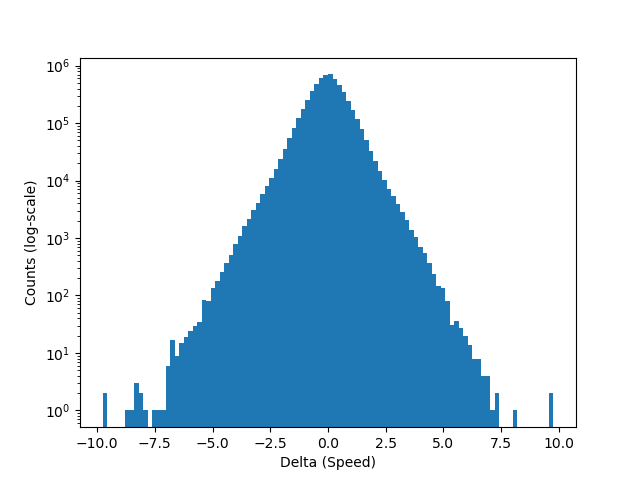
\includegraphics[width=0.6\linewidth]{figs/nedit_speed_distr.png}
  \vspace{0.1in}
  \label{fig:ne_speed_distr}
\end{figure*}

~\Cref{tab:neural-editor-eval} shows the results of training. We run all training scenarios three times and take the average. We find that all modifications significantly change the resulting $\Delta$ value while generally preserving lexical and semantic similarity. The variance across test samples is relatively low for each metric (\eg $0.005$ for BERTScore) so we only report the averaged metric. Unsurprisingly, when tolerance is low, we find good performance in $\Delta$ and poor performance in the similarity metrics. This result is likely due to overfitting from the lack of large amounts of training data. We see the strongest results with the Perturbation \& $\Delta$-Tolerance approaches, indicating that combining the two approaches is beneficial when the tolerance is tuned. 

At tolerance $\epsilon = 0.05$, including perturbed edit vectors improves the similarity metrics at the cost of $\Delta$, indicating that the perturbed approach may help combat overfitting. With tolerance $\epsilon = 0.1$, we see that perturbation is generally not helpful, and surprisingly, at tolerance $\epsilon = 0.2$, the perturbation approach leads to a higher $\Delta$. We hypothesize that at tolerance $\epsilon = 0.2$, there is an effective balance of constraint to a certain $\Delta$ and enough data for robust training. Further, the perturbation likely benefits from having $\Delta$-constrained pairs. We leave it to future work to investigate this behavior.

\begin{table}[h]
  \centering
  \small
  \caption{Evaluation metrics (BLEU \citep{Papineni2002bleu} and BERTScore \citep{zhang2019bertscore}) and strength of control on $\Delta$ for the trained models (ideally, $\Delta = 0.5$). The scores are averaged across three training runs with different seeds. We train a baseline model \citep{guu2018generating} (NeuralEditor Baseline), as well as multiple variants of the baseline. Neighborhood creation models are listed as ``Tol=$\epsilon$'' where $\epsilon$ is the tolerance. We also train a model following the edit vector perturbation approach and multiple models combining the two approaches. }
  \label{tab:neural-editor-eval}
  \begin{tabularx}{0.9\linewidth}{@{}>{\raggedright\arraybackslash}Xcccc@{}}
   \toprule[1.5pt]
  \textsc{Model} & \textsc{Delta} & \textsc{Train BLEU} & \textsc{Test BLEU} & \textsc{BERTScore} \\     
  \midrule[0.75pt]
  % \addlinespace[0.5em]
\textsc{NeuralEditor} Baseline    & 0.0113 & \textbf{0.6691}     & \textbf{0.5679}    & 0.9327 \\
  \midrule[0.75pt]
Tol=0.05               & 0.4559 & 0.8057     & 0.4266    & 0.9326 \\
Tol=0.1                & 0.4558 & 0.7146     & \textbf{0.5747}    & 0.9340 \\
Tol=0.2                & 0.4405 & 0.5994     & 0.5628    & 0.9355 \\
  \midrule[0.75pt]
Perturbation            & 0.4433 & 0.5513     & 0.4531    & 0.9346 \\
Perturbation + Tol=0.05 & 0.4279 & 0.5709     & 0.5218    & 0.9329 \\
Perturbation + Tol=0.1  & 0.4355 & 0.6375     & 0.5100    & 0.9386 \\
Perturbation + Tol=0.2  & \textbf{0.4596} & \textbf{0.6751}     & \textbf{0.5679}    & 0.9334 \\
  \bottomrule[1.5pt]\\
  \end{tabularx}
  \vspace{-10pt}
  \end{table}

\Cref{tab:ne_example} shows the generations of the \textsc{NeuralEditor} Baseline and each method with the tolerance at $0.2$. For both sequences, the generations of our modified models are much shorter while preserving content, indicating higher speed. The baseline for both prompts made minimal edits to the input sentences (\eg ``excellent'' to ``amazing''), resulting in close to no change in speed but an extremely high similarity. 

  \begin{table}[htb]
  \small
  \centering
  \caption{The baseline \citep{guu2018generating} (Prototype-then-Edit) as well as multiple variants of the baseline. Neighborhood creation models are listed as ``Tol=$\epsilon$'' where $\epsilon$ is the tolerance. The models are fed the input (\ie \textbf{Original}) and generate by applying an ``edit vector'' to the latent representation of the input sentence.}
  \label{tab:ne_example} 
  \begin{tabularx}{\linewidth}{@{}>{\raggedright\arraybackslash}X@{}}
   \toprule[1.5pt]
  \textsc{Model} \& \textsc{Generated Text}\\
  \midrule[0.75pt]
  \textsc{Example 1:}\\
  \textbf{Original}: He went above and beyond in providing us excellent customer service and was extremely courteous friendly and kind.  \\
  \textbf{\textsc{NeuralEditor} Baseline}: He went above and beyond in providing us with amazing customer service and was extremely courteous friendly and kind.  \\
  \textbf{Tol=0.2}: Always amazing customer service and very knowlegable staff. \\
  \textbf{Perturbation + Tol=0.2}: He was knowledgable, courteous, and went provided excellent customer service.\\
  \addlinespace[0.5em]
  \textsc{Example 2:}\\
  \textbf{Original}: The staff is very professional and friendly \& environment is clean.  \\
  \textbf{\textsc{NeuralEditor} Baseline}: The staff is very professional and likable \& the environment is clean. \\
  \textbf{Tol=0.2}: The friendly staff is very professional \& environment is clean. \\
  \textbf{Perturbation + Tol=0.2}: Friendly staff and clean environment.\\
  \bottomrule[1.5pt]\\
  \end{tabularx}
  \vspace{-10px}
  \end{table}

While the architecture shows a strong control over speed, it is hard to adjust our formulation to a wide range of controls. Neighborhood creation can easily be adapted for any control but severely restricts the amount of training data. Perturbation works well with constraints defined with word embeddings due to how the edit vector is constructed, but it likely will struggle with other controls. 

For traits like persuasiveness, we mainly enforce controls with a learned classifier or many smaller constraints (\eg speed). In the case of the former, this architecture would likely struggle because it would not have access to the learned weights. For the latter, having many constraints would limit the size of the training data and pollute the edit vector perturbation. We look to other models to resolve these issues.

In this section, we adapt the prototype-then-edit model proposed by \citet{guu2018generating} to controllable text generation. We show that our approach leads to significant control over speed while preserving relevance to the original text. In the next section, we modify the adversarial framework from~\Cref{chp:style_infusion} to control the speed of generated text and compare the results against this section's approach.

% Example 1
% he went above and beyond in providing us excellent customer service and was extremely courteous friendly and kind. 
% always amazing customer service and very knowlegable staff.
% he was knowledgable, courteous, and went provided excellent customer service.

% Example 2
% the staff is very professional and friendly & environment is clean.
% the friendly staff is very professional & environment is clean.
% friendly staff and clean environment.

